\documentclass[11pt,a4paper]{article}

\usepackage[utf8]{inputenc}
\usepackage[T1]{fontenc}
\usepackage{amsmath, amssymb}
\usepackage{geometry}
\usepackage{xcolor}
\usepackage{tikz}
\usetikzlibrary{decorations.pathreplacing}
\usepackage{mdframed}

\geometry{margin=2.5cm}

\newcommand{\R}{\mathbb{R}}

\title{\textbf{Encodage one-hot des séquences}\\
\large Décomposition de \texttt{np.eye(A, dtype=np.float32)[sequences]}}
\author{Institut de la Vision --- Directed Evolution Loop}
\date{}

\begin{document}
\maketitle

% ─────────────────────────────────────────────────────────────────────────────
\section{Le code}

\begin{verbatim}
sequences_arr = np.asarray(sequences)
N_seqs        = sequences_arr.shape[0]
X             = np.eye(A, dtype=np.float32)[sequences]  # shape (N, L, A)
return X.reshape(N_seqs, L*A)
\end{verbatim}

Ce code transforme une librairie de $N$ séquences de longueur $L$ (chacune une
suite d'indices d'acides aminés dans $\{0,\ldots,A-1\}$) en une matrice de
caractéristiques \emph{one-hot} de taille $(N, L\cdot A)$, prête à être utilisée
comme matrice de design $X$ dans \texttt{build\_potts\_features}.

% ─────────────────────────────────────────────────────────────────────────────
\section{Étape par étape}

\subsection*{Étape 1 : \texttt{np.asarray(sequences)}}
Convertit \texttt{sequences} (qui peut être une liste, un tableau JAX, etc.) en
un tableau NumPy standard, de forme $(N, L)$, à valeurs entières dans
$\{0,\ldots,A-1\}$. C'est purement une conversion de type ; aucune donnée n'est
modifiée.

\subsection*{Étape 2 : \texttt{np.eye(A, dtype=np.float32)}}
Construit la matrice identité $A\times A$ :
\[
    I_A =
    \begin{pmatrix}
        1 & 0 & \cdots & 0 \\
        0 & 1 & \cdots & 0 \\
        \vdots & & \ddots & \vdots \\
        0 & 0 & \cdots & 1
    \end{pmatrix} \in \R^{A\times A}.
\]
La ligne $k$ de $I_A$ est le vecteur one-hot de l'acide aminé $k$ : que des
zéros, sauf un $1$ en position $k$.

\subsection*{Étape 3 : indexation \texttt{[sequences]}}
C'est l'étape la moins évidente. NumPy interprète \texttt{sequences} (un
tableau d'entiers de forme $(N, L)$) comme un tableau d'\emph{indices de
lignes} à extraire de $I_A$. Pour chaque entrée \texttt{sequences[n, l]} $= k$,
NumPy va chercher la ligne $k$ de $I_A$ et la place à la position $(n, l)$ du
résultat. Le résultat a donc une dimension de plus que l'entrée :
\[
    \underbrace{I_A}_{(A,A)}\big[\underbrace{\texttt{sequences}}_{(N,L)}\big]
    \;\longrightarrow\;
    \underbrace{X}_{(N, L, A)}
    \qquad\text{avec}\qquad
    X[n, l, :] = I_A[\texttt{sequences}[n,l], :].
\]
Autrement dit : pour chaque séquence $n$ et chaque position $l$, on obtient le
vecteur one-hot (de longueur $A$) de l'acide aminé qui s'y trouve.

\subsection*{Étape 4 : \texttt{X.reshape(N\_seqs, L*A)}}
On aplatit les deux dernières dimensions $(L, A)$ en une seule de taille
$L\cdot A$, en concaténant les $L$ blocs one-hot les uns à la suite des autres.
Chaque ligne de la matrice finale est donc un vecteur creux de longueur
$L\cdot A$, avec exactement $L$ entrées à $1$ (une par position) et le reste à
$0$.

% ─────────────────────────────────────────────────────────────────────────────
\section{Schéma}

L'exemple ci-dessous utilise $L=3$ positions et $A=5$ acides aminés (au lieu de
$L=7$, $A=20$ dans le code réel) pour que le schéma tienne sur la page. La
séquence $s = (2, 0, 4)$ signifie : acide aminé $2$ en position $0$, acide
aminé $0$ en position $1$, acide aminé $4$ en position $2$.

\begin{center}
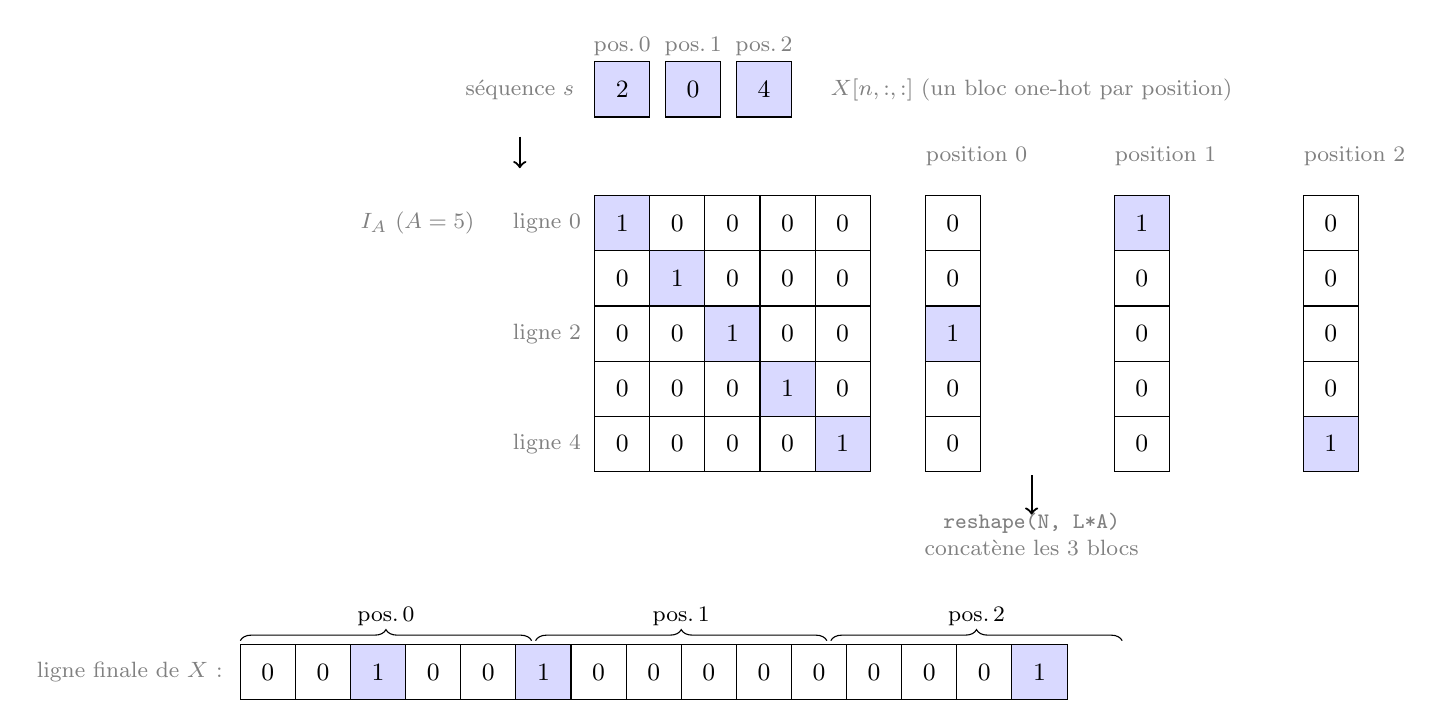
\begin{tikzpicture}[
    cellA/.style={draw, minimum width=0.7cm, minimum height=0.7cm, font=\small},
    cellHL/.style={draw, fill=blue!15, minimum width=0.7cm, minimum height=0.7cm, font=\small},
    lbl/.style={font=\footnotesize, text=gray},
]

% ---- Séquence d'entrée ----
\node[lbl] at (-1.3,4.6) {séquence $s$};
\foreach \i/\val in {0/2, 1/0, 2/4} {
    \node[cellHL] (seq\i) at (\i*0.9, 4.6) {\val};
}
\node[lbl] at (0*0.9,5.15) {pos.\,0};
\node[lbl] at (1*0.9,5.15) {pos.\,1};
\node[lbl] at (2*0.9,5.15) {pos.\,2};

% ---- Flèche vers I_A ----
\draw[->, thick] (-1.3,4.0) -- (-1.3,3.6) node[midway, right, font=\footnotesize] {};

% ---- Matrice identité I_A (A=5) ----
\node[lbl] at (-2.6,2.9) {$I_A$ ($A=5$)};
\foreach \r in {0,...,4} {
    \foreach \c in {0,...,4} {
        \pgfmathtruncatemacro{\ishit}{\r==\c}
        \ifnum\ishit=1
            \node[cellHL] at (\c*0.7, 2.9-\r*0.7) {1};
        \else
            \node[cellA] at (\c*0.7, 2.9-\r*0.7) {0};
        \fi
    }
}
\node[lbl, anchor=east] at (-0.4, 2.9-0*0.7) {ligne 0};
\node[lbl, anchor=east] at (-0.4, 2.9-2*0.7) {ligne 2};
\node[lbl, anchor=east] at (-0.4, 2.9-4*0.7) {ligne 4};

% ---- Résultat X (N,L,A) : 3 blocs one-hot ----
\node[lbl] at (5.2,4.6) {$X[n,:,:]$ (un bloc one-hot par position)};
\foreach \pos/\aa/\xoff in {0/2/4.2, 1/0/6.6, 2/4/9.0} {
    \node[lbl] at (\xoff+0.3,3.75) {position \pos};
    \foreach \k in {0,...,4} {
        \pgfmathtruncatemacro{\ishit}{\k==\aa}
        \ifnum\ishit=1
            \node[cellHL] at (\xoff, 2.9-\k*0.7) {1};
        \else
            \node[cellA] at (\xoff, 2.9-\k*0.7) {0};
        \fi
    }
}

% ---- Flèche reshape ----
\draw[->, thick] (5.2,-0.3) -- (5.2,-0.8);
\node[lbl, align=center] at (5.2,-1.05) {\texttt{reshape(N, L*A)}\\ concatène les 3 blocs};

% ---- Vecteur final aplati (L*A = 15) ----
\foreach \i in {0,...,14} {
    \pgfmathparse{Mod(\i,5)}
    \let\localaa\pgfmathresult
    \pgfmathparse{int(\i/5)}
    \let\localpos\pgfmathresult
    \pgfmathtruncatemacro{\ison}{(\localpos==0 && \localaa==2) || (\localpos==1 && \localaa==0) || (\localpos==2 && \localaa==4)}
    \ifnum\ison=1
        \node[cellHL] at (\i*0.7-4.5,-2.8) {1};
    \else
        \node[cellA] at (\i*0.7-4.5,-2.8) {0};
    \fi
}
\draw[decorate,decoration={brace,amplitude=4pt}] (-4.85,-2.4) -- (-1.15,-2.4) node[midway,above,font=\footnotesize,yshift=2pt]{pos.\,0};
\draw[decorate,decoration={brace,amplitude=4pt}] (-1.1,-2.4) -- (2.6,-2.4) node[midway,above,font=\footnotesize,yshift=2pt]{pos.\,1};
\draw[decorate,decoration={brace,amplitude=4pt}] (2.65,-2.4) -- (6.35,-2.4) node[midway,above,font=\footnotesize,yshift=2pt]{pos.\,2};
\node[lbl, anchor=east] at (-4.95,-2.8) {ligne finale de $X$ :};

\end{tikzpicture}
\end{center}

Les cases bleutées marquent les $1$ (une seule par position) ; toutes les
autres cases valent $0$. La ligne finale contient exactement $L=3$ uns sur
$L\cdot A = 15$ entrées --- un vecteur \textbf{creux} (\emph{sparse}) : dans le
code réel, $L=7$ et $A=20$, donc chaque ligne ne compte que $7$ entrées non
nulles sur $140$ (et, une fois les termes de paires ajoutés, $7+21+1=29$ entrées
non nulles sur $8541$).

% ─────────────────────────────────────────────────────────────────────────────
\section{Résumé}

\begin{mdframed}
\texttt{np.eye(A)[sequences]} exploite l'indexation \emph{fancy indexing} de
NumPy : indexer la matrice identité par un tableau d'entiers revient à
sélectionner, pour chaque entier, la ligne correspondante de l'identité ---
c'est-à-dire son vecteur one-hot. Appliqué à un tableau de séquences $(N, L)$,
cela produit directement un tenseur $(N, L, A)$ de vecteurs one-hot, un par
position et par séquence, sans boucle Python explicite. Le \texttt{reshape}
final aplatit ces $L$ blocs en une seule ligne de taille $L\cdot A$ par
séquence --- exactement la représentation attendue par la régression Ridge
sur les caractéristiques de Potts.
\end{mdframed}

\end{document}
